\documentclass{jot}
% Use the documentclass option 'lineno' to view line numbers

% Enter the JOT metadata in the following 
\usepackage{multirow}

\jotdetails{
    volume=vv,      % volume
    number=nn,       % number or issue
    articleno=aa,   % article number, eg a1 for research articles, e for editorials
    year=2022,      % year
    license=ccby    % choose from ccby, ccbynd, ccbyncnd
}
\newcommand{\command}[1]{{\color{codepurple}\texttt{\textbackslash #1}}}
\newcommand{\param}[1]{{\color{blue}\texttt{#1}}}
% Select the article type
\articletype{regular} 
    % {editorial} editorial 
    % {regular} regular contribution
    % {manual} manual
    % {column} column

\title{Towards behavioral consistency in multi-modeling}

\author[$\ast$]{Tim Kräuter}
% Arbitrary co-author order. Everyone contributed significantly.
\author[$\ast\dagger$]{Harald König}
\author[$\ast$]{Adrian Rutle}
\author[$\ast$]{Yngve Lamo}
\author[$\ddagger$]{Patrick Stünkel}

\affil[$\ast$]{Western Norway University of Applied Sciences, Bergen, Norway}
\affil[$\dagger$]{University of Applied Sciences, FHDW, Hannover, Germany}
\affil[$\ddagger$]{Haukeland Universitetssykehus, Bergen, Norway}

\keywords{	
Global behavioral consistency,
Consistency verification,
Multi-modeling,
Graph transformation,
Heterogeneous models
}

\runningtitle{Towards behavioral consistency in multi-modeling} % For use in the internal pages 

\runningauthor{Kräuter \textit{et al.}}

\usepackage{amsthm} % for proofs
\usepackage{amsmath} % theorems, definitions, etc.
\newtheorem{definition}{Definition}
\newcommand{\definitionautorefname}{Definition}

% Table

\usepackage{glossaries}
\usepackage{cleveref} % Reference footnotes.
\crefformat{footnote}{#2\footnotemark[#1]#3}

\newacronym{ltl}{LTL}{Linear temporal logic}
\newacronym{mde}{MDE}{Model-driven engineering}
\newacronym{bpmn}{BPMN}{Business Process Modeling Notation}
\newacronym{uml}{UML}{Unified Modeling Language}
\newacronym{csp}{CSP}{Communication Sequential Processes}
\newacronym{ccsl}{CCSL}{Clock Constraint Specification Language}

% correct bad hyphenation here
\hyphenation{be-ha-vi-o-ral}

\begin{abstract}
%ABOUT: Introduce multi-model and motivate global behavior checking
Multiple interacting systems are needed to realize the requirements of complex domains.
Describing the interactions between these systems and checking their global behavioral consistency is a general, well-known challenge in software engineering.
To address this challenge, model-driven software engineering utilizes abstract representations of the constituting systems and their interactions, resulting in a \emph{multi-model} representing the overall software.
In such a multi-modeling setting, global consistency rules must be satisfied by a set of heterogeneously typed models to guarantee a desired \emph{global behavior}.
In this paper, we propose a novel approach for behavioral consistency management of heterogeneous multi-models.
The approach introduces a workflow in which we
(i) align the individual models and specify their \emph{interactions}, 
(ii) generate a \emph{global execution semantics} for the multi-model, and finally,
(iii) define and check \emph{global properties} which should be satisfied by the multi-model.
Although our approach is independent of a particular formalism as an underlying global execution semantics, the current implementation utilizes graph transformations for this purpose.
\end{abstract}

% TODO: Comment in after acceptance and helpful feedback.
% \acknowledgment{We want to thank the anonymous reviewers for their valuable comments and helpful suggestions.}

\begin{document}    
\maketitle
\urlstyle{rm}

\section{Introduction}
% Introduce multi-model
\gls*{mde} addresses the increasing complexity of software systems by employing models to describe the different aspects of the system.
In this way, \gls*{mde} promotes a clear separation of concerns and raises the abstraction level throughout the entire development process \cite{franceModeldrivenDevelopmentComplex2007}.
These models are then used to generate portions of the system leading to an increase in productivity and reduction of errors \cite{brambillaModeldrivenSoftwareEngineering2017}.
As multiple interacting systems are needed to realize the requirements of complex domains, a set of corresponding models would be needed to represent these systems and their interactions.
Such a collection of inter-related models is referred to as a \emph{multi-model} \cite{boronatWhatMultimodelingLanguage2009, stunkelComprehensiveSystemsFormal2021}, which is usually heterogeneous, meaning it consists of models conforming to different modeling languages.
% Consistency in multi-modeling
Models in a multi-model contradicting each other can lead to problems during development, system generation, and system execution.
Consequently, continuous multi-model consistency management during the development process is a significant issue for multi-models \cite{spanoudakisInconsistencyManagementSoftware2001, cicchettiMultiviewApproachesSoftware2019}.

% Consistency can be checked for a set of structural models
Recent research describes methods to check the structural consistency of a multi-model \cite{stunkelComprehensiveSystemsFormal2021, klareCommonalitiesPreservingConsistency2019}.
Structural models, like UML class diagrams, describe structural aspects of systems, i.e., domain concepts and relations between these concepts.
This is usually referred to as the static semantics of the software system as it only describes the set of valid instances or states of the system.
% Challenge: Consistency for a set of behavioral models.
Nevertheless, approaches to multi-model consistency management must also include a means to maintain \emph{behavioral consistency} since behavioral models, like \gls*{bpmn}, are associated with execution semantics describing dynamic aspects of the system \cite{objectmanagementgroupUnifiedModelingLanguage2017, objectmanagementgroupBusinessProcessModel2013}.

% Existing solutions. But they are not sufficient!
Several approaches exist for checking the consistency of pairs of behavioral models.
For example, consistency checking for sequence diagrams and statecharts was implemented using Petri nets \cite{yaoConsistencyCheckingUML2006} and \gls*{csp} \cite{kusterExplicitBehavioralConsistency2003}.
Moreover, some approaches for model simulation in heterogeneous scenarios have been developed, such as Ptolemy \cite{ekerTamingHeterogeneityPtolemy2003, leeDisciplinedHeterogeneousModeling2010} and GEMOC studio \cite{deantoniModelingBehavioralSemantics2016, varalarsenBCoolBehavioralCoordination2016}.
However, current approaches either only allow for consistency checking of two behavioral models or do not allow for definition and checking of global behavioral properties.

% % Our approach summarized.
We propose a novel approach for consistency management of heterogeneous multi-models, which allows us to define and check \emph{global} behavioral properties.
Our approach allows specifying \emph{interactions} between potentially heterogeneous behavioral models, which are in turn used to generate global execution semantics.
Although our approach is independent of a particular formalism as an underlying global execution semantics, the current implementation utilizes the rewriting logic tool Maude (see \autoref{sec:maude_execution_semantics}).

% Paper outline
The remainder of this paper is structured as follows.
We introduce a simplified use case (\autoref{sec:usecase}) before explaining our behavioral consistency management approach in detail (\autoref{sec:behavioral_consistency_checking}).
Afterward, we show how we can use the Maude system based on equational and rewriting logic as execution semantics (\autoref{sec:maude_execution_semantics}).
Finally, we discuss related work in \autoref{sec:related_work} and conclude in \autoref{sec:conclusion_and_future_work}.

\section{Use Case} \label{sec:usecase}
This section motivates our approach by a simplified use case in which a traffic management system is developed to guide the traffic at a T-Junction with three traffic lights.
It should lead the traffic by switching between the two traffic phases highlighted in \autoref{fig:junction-phases}.
In addition, the system must fulfill the following two requirements.
First, it must guarantee safe traffic by changing the three traffic lights, A, B, and C, correctly.
Second, it should prioritize arriving buses, i.e., switch the traffic lights quicker than usual to let an approaching bus pass (early green).
This so-called bus priority signal is a widely implemented technique to improve service and reduce delays in public transport.

\begin{figure}[h]
    \centering
    % warning is fine since it does not visually overflow.
    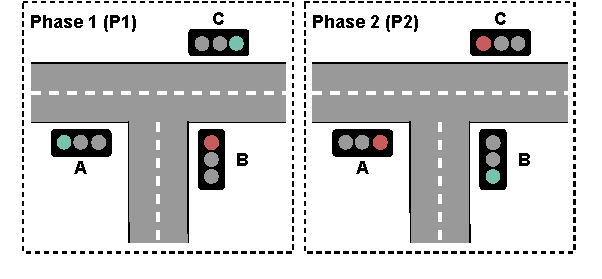
\includegraphics[width=0.5\textwidth]{figures/phases.pdf}
    \caption{Traffic phases of a T-Junction}
    \label{fig:junction-phases}
\end{figure}

To develop the behavior of the traffic management system, we follow an \gls*{mde} approach.
First, we model the behavior of a traffic light as a \gls*{uml} state machine, and then we use \gls*{bpmn} to model the different traffic phases of the T-Junction, including the prioritization of approaching buses.

Using different behavioral modeling languages in the use case has two reasons.
First, two software development teams might work on the system in parallel but prefer different modeling languages.
Second, each team is free to choose the most appropriate modeling language for defining their part of the system.
In this use case, the behavior of a traffic light and a T-Junction differs significantly in complexity and requirements, resulting in the use of two different behavioral modeling languages, namely \gls*{uml} state machines, and \gls*{bpmn}.

The behavior of a traffic light is straightforward since it uses only three colors to guide the traffic.
\autoref{fig:trafficLight} shows the typical European\footnote{Traffic lights in other parts of the world might not show red and amber simultaneously before switching to green.} traffic light that switches from \textsf{red} to \textsf{red-amber}, \textsf{green}, \textsf{amber}, and back to \textsf{red}.
The start state of the traffic light in \autoref{fig:trafficLight} is \textsf{red} but can be any of the four possible states.

\begin{figure}[h]
    \centering
    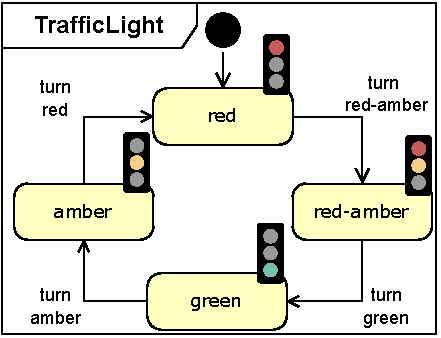
\includegraphics[width=0.35\textwidth]{figures/trafficLight.pdf}
    \caption{Traffic light state machine model}
    \label{fig:trafficLight}
\end{figure}

However, the T-Junction's behavior is more complex since it should coordinate the three traffic lights and communicate with approaching buses to implement bus priority.
Consequently, we are using \gls*{bpmn} to model this aspect of the system's behavior since we can utilize \gls*{bpmn} message and signal events to implement the communication with approaching buses.

We model two processes, one for the T-Junction and the Bus.
Each process is modeled in its own \gls*{bpmn} \emph{pool}.
A pool is depicted as a vertical lane with a name on the left and allows to draw message flows (arrows with dashed lines) between two different pools.

\autoref{fig:t_junction} shows how a possible controller for a T-Junction behaves in the traffic management system\footnote{All models and their source files can be found at \cite{timkrauterBehavioralConsistencyMultimodeling2022}.\label{footnote:fullModels}}.
When a T-Junction controller is started, we assume that the traffic lights are showing the colors according to phase 1 (see \autoref{fig:junction-phases}).
Thus, the controller enters a subprocess called phase 1, which we describe later.
However, when a fixed amount of time has passed, the subprocess is interrupted by the attached timer boundary event.
Then, the controller executes the next activity and switches to phase 2.
The controller will pass a throwing signal event before entering a subprocess for phase 2 and repeat the same steps.
This signal event represents a broadcast to all buses waiting for traffic light B to become green.
After switching back from phase 2 to phase 1 and signaling that traffic lights A and C are green, the controller can stop or execute the described steps again.
Typically, the controller does not stop, which is indicated by the default sequence flow going back to the process beginning.

% T-Junction BPMN model
\begin{figure*}[h]
    \centering
    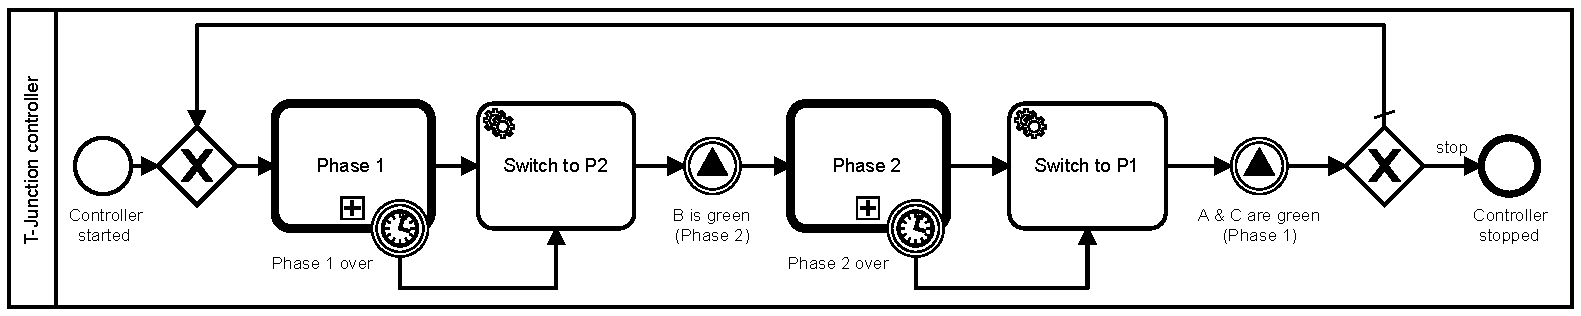
\includegraphics[width=1\textwidth]{figures/t-junction.pdf}
    \caption{Model for a T-Junction controller}
    \label{fig:t_junction}
\end{figure*}

% Bus and Phase 1 BPMN model
\begin{figure*}[h]
    \centering
    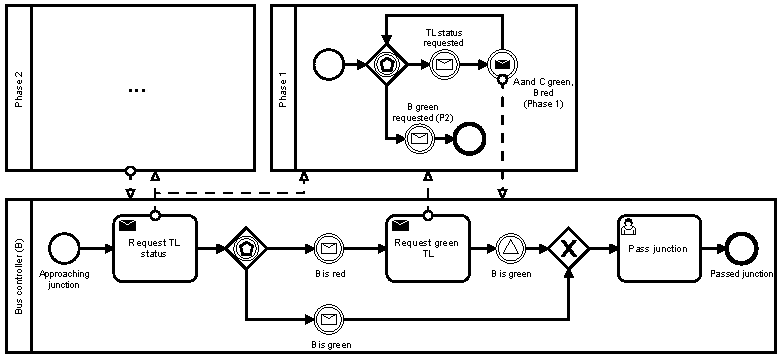
\includegraphics[width=1\textwidth]{figures/communication.pdf}
    \caption{Model for a bus with direction B and its communication with a T-Junction}
    \label{fig:communication}
\end{figure*}

\autoref{fig:communication} shows the communication of a bus with the subprocess phase 1.
The \gls*{bpmn} model and communication for phase 2 of the controller can be defined accordingly \cref{footnote:fullModels}.

The phase 1 model uses an event-based gateway to respond to two different kinds of messages.
First, the traffic light status can be requested, which is answered by sending a message declaring that the traffic lights A and C are green while B is red.
Moreover, early green for traffic light B  can be requested.
This request ends the subprocess, and the controller immediately switches to phase 2 (see \autoref{fig:t_junction}), which results in the traffic light B turning green.

The bottom of \autoref{fig:communication} shows the controller for a bus parameterized with direction B.
It will first request the traffic light status to determine if traffic light B is green.
If it is green, the bus can pass the junction.
However, if it is red, the bus requests to change B to green and waits for a signal that the controller has changed the traffic light.
After receiving the signal, the bus passes the junction.
In addition, the bus controller also communicates with the phase 2 subprocess, which we only hint at in \autoref{fig:communication}\cref{footnote:fullModels}.
A \gls*{bpmn} model for a bus controller parameterized with the direction A or C looks nearly identical.

Having developed behavioral models for the system, we want to check the previously stated \emph{safe traffic} requirement while buses are prioritized.
We can lower the overall development cost if we find bugs related to these requirements as early as possible during system development.
However, the traffic light model is currently not related to the T-Junction and bus models, which is a problem since the T-Junction is supposed to control the traffic lights, for example, when it switches between the two traffic phases.
In addition, the system has to manage multiple slightly different instances of the behavioral models.
For example, there are three traffic lights at one T-Junction starting in different states, i.e., showing different colors and buses approaching the T-Junction from one of the three directions.
Consequently, we need a model of the system to allow us to define interactions between the models and configure instances of the behavioral models contained in the multi-model.

The resulting model called the \emph{system relationship model} is shown in \autoref{fig:systemRelationshipMetamodel} using a class diagram-like syntax.
It contains one class for each behavioral model and associations to depict behavioral relationships, leading to possible interactions.
In addition, it contains enumerations to parameterize the behavioral models.

\begin{figure}[h]
    \centering
    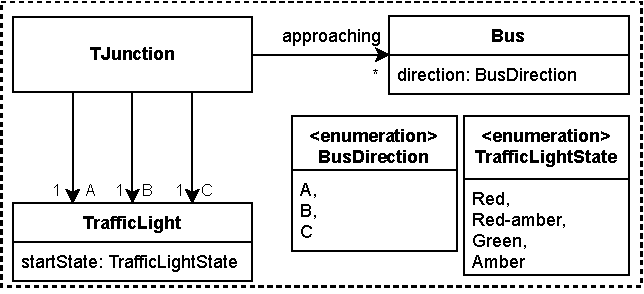
\includegraphics[width=0.45\textwidth]{figures/systems.pdf}
    \caption{System relationship model of the traffic management system}
    \label{fig:systemInteractionModel}
\end{figure}

A \textsf{TJunction} has three associated \textsf{TrafficLight}s, A, B, and C, and a set of currently approaching \textsf{Bus}es.
A \textsf{TrafficLight} has four possible \textsf{TrafficLightState}s and an attribute to define its \textsf{startState}.
A \textsf{Bus} has a \textsf{direction} that indicates which \textsf{TrafficLight} of the T-Junction it is approaching.

Finally, using the system relationship model, we can define a test configuration of our traffic management system to check its requirements.
\autoref{fig:test_config} depicts the test system configuration, an instance of the system relationship model.
First, it contains three instances of the traffic light behavioral model, representing the three traffic lights, \textbf{A}, \textbf{B}, and \textbf{C}.
Second, it contains an instance of the T-Junction behavioral model, which is connected to the three traffic lights, and two instances of the bus behavioral model.
Thus, the test system configuration describes a system that controls one T-Junction with three traffic lights and two buses approaching from directions A and C.

\begin{figure}[h]
    \centering
    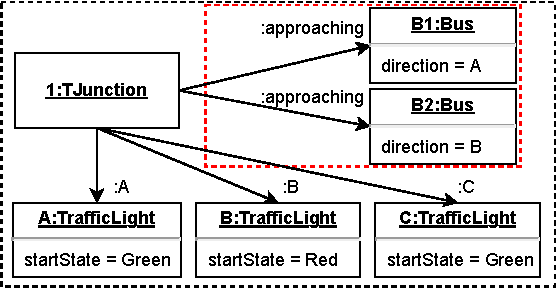
\includegraphics[width=0.45\textwidth]{figures/test_config.pdf}
    \caption{Test system configuration}
    \label{fig:test_config}
\end{figure}

First, we would like to check the safe traffic requirement.
Since we only want to check system conformance concerning the two traffic phases, we do not need to include the two buses depicted in the red dotted square in \autoref{fig:test_config} in the analysis.
We cannot simply assert that the system is either in phase 1 or phase 2 since there are intermediate states during the transition between the two phases, which are allowed.
By consulting \autoref{fig:trafficLight}, we can, for example, expect a state in which traffic lights A and C are amber, and traffic light B is red-amber before reaching phase 2.
However, we can define \emph{safe traffic} as the absence of \emph{unsafe traffic}, which is easier to define.

For the T-Junction, unsafe traffic occurs if traffic light A is green or amber and traffic light B is green or amber simultaneously.
In addition, the same state combinations are forbidden for traffic lights B and C.
We can formalize the consistency requirements as safety properties in \gls*{ltl}, i.e., states that should never be reached.
The resulting global properties \ref{eq:property1} and \ref{eq:property2}\footnote{We assume the existence of atomic propositions for each traffic light showing the color green or amber. The propositions are formalized later.} are the following:
\begin{align}
    \square\neg((A_{green} \lor A_{amber}) \land (B_{green} \lor B_{amber})) \label{eq:property1} \\
    \square\neg((C_{green} \lor C_{amber}) \land (B_{green} \lor B_{amber})) \label{eq:property2}
\end{align}

If we include buses \textsf{B1} and \textsf{B2} in the system, we would like to check that they cannot pass when their traffic light is red or red-amber.
Concretely, this means the \textsf{Pass Junction} activity should not execute while the corresponding traffic light is \textsf{red} or \textsf{red-amber}.
We formalize these requirements again by using \gls*{ltl} safety properties \ref{eq:property3} and \ref{eq:property4}\footnote{The atomic proposition $B1_{passing}\, / \,B2_{passing}$ represents that \textsf{Pass Junction} (see \autoref{fig:communication}) has started but not finished yet, i.e., there is a token in the activity when using \gls*{bpmn} token semantics \cite{objectmanagementgroupBusinessProcessModel2013}.}.

\begin{align}
    \square\neg(B1_{passing} & \land (A_{red} \lor A_{red-amber})) \label{eq:property3} \\
    \square\neg(B2_{passing} & \land (B_{red} \lor B_{red-amber})) \label{eq:property4}
\end{align}

However, to check the global properties, we must execute the system with the behavior specified in the behavioral models according to the test configuration.
This is not straightforward since the multi-model of the use case consists of a system relationship model relating two heterogeneous behavioral models.
In addition, the system configuration instantiates two of the behavioral models multiple times with different parameters.
Furthermore, we face the problem that the models are not independent of each other.
For example, the T-Junction controller must control when the traffic lights A, B, and C switch their states.
Thus, if we were to run the models independently in parallel, the properties would be violated.

Current approaches can only simulate a set of interacting heterogeneous behavioral models.
However, they do not allow multiple instances of a behavioral model (without duplicating it) nor provide concrete means to define and check \emph{global} behavioral properties.
Thus, they are not capable of checking multi-model behavioral consistency.
A multi-model is behaviorally consistent if it satisfies all of its behavioral properties.
A behavioral property is given in temporal logic, for example, \gls*{ltl} earlier, and is characterized as \emph{local} if it constrains only one model and as \emph{global} if it spans two or more models in a multi-model.
Furthermore, global properties are dependent on the system configuration, i.e., the instance of the system relationship model used.
In the remainder of this paper, we will describe our approach to address behavioral consistency in multi-modeling and apply it to this use case.

\section{Behavioral consistency management} \label{sec:behavioral_consistency_checking}
% Introduce the overall approach using the workflow somehow here and follow it.
\autoref{fig:approach} depicts our approach to behavioral consistency management using a \gls*{bpmn} diagram.
We leave potential consistency restoration as a problem for future work.

\begin{figure}[h]
    \centering
    % https://cawemo.com/share/3323b181-61ec-4d73-a7cc-6ffccf4204dc
    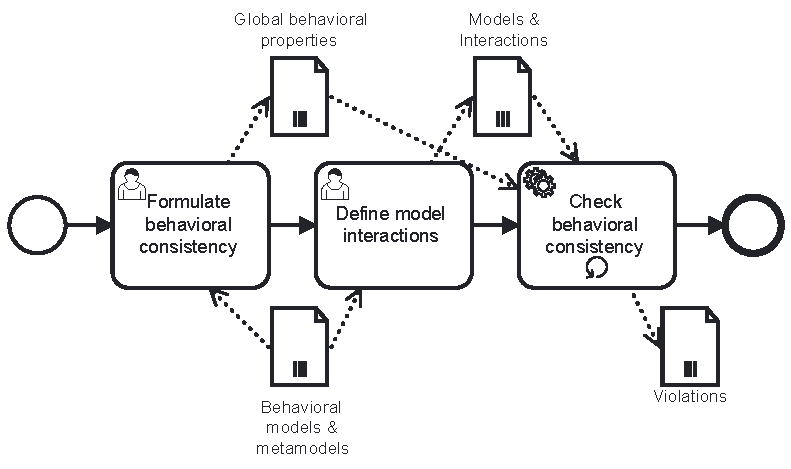
\includegraphics[width=0.475\textwidth]{figures/workflow.pdf}
    \caption{Behavioral consistency management workflow}
    \label{fig:approach}
\end{figure}

Our approach can be summarized in three steps.
First, we define interactions between the behavioral models, which describe parts of a system.
Second, based on these interactions and the behavioral models, we generate execution semantics for the global system.
Finally, given a system configuration and consistency requirements, we can check these requirements using the generated global execution semantics.

We will now describe our approach in detail by introducing the different model types and explaining each step separately.

\subsection{Prerequisites}
As prerequisites, we assume a set of behavioral models, including their metamodels, see \autoref{fig:modelTypes}.
In addition, we require a snapshot metamodel for each behavioral metamodel used.
A snapshot metamodel should represent the structure of a state for a given behavioral language, defined in a metamodel.
For example, each state in a Petri net is defined by a set of tokens distributed over its places.

\begin{figure}[h]
    \centering
    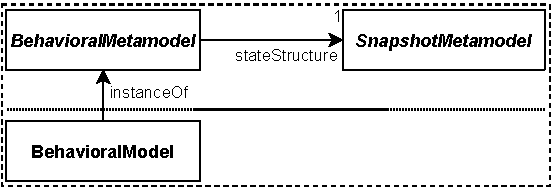
\includegraphics[width=0.45\textwidth]{figures/modelTypes.pdf}
    \caption{Behavioral metamodels and snapshot metamodels}
    \label{fig:modelTypes}
\end{figure}

Furthermore, we will later introduce the system relationship model, which is used to define behavioral relationships between the behavioral models.
We will now explain the different model types in detail and give examples of them for the use case.

\subsubsection{Metamodels}
Each behavioral model must conform to a metamodel (see \autoref{fig:modelTypes}).
A metamodel can be defined by a class diagram/grammar for graphical/textual modeling languages.
The metamodel ensures that the corresponding models are machine-readable, which is crucial when automating parts of the consistency checking.

The use case utilizes state machine and \gls*{bpmn} models.
\autoref{fig:fsm_metamodel} shows the metamodel for finite state machines (ignore the purple coloring for now).
It is defined by a \gls*{uml} class diagram with additional information depicted in clouds.
The clouds define a concrete syntax for state machines inspired by \gls*{uml} statecharts.
A model in this concrete syntax, such as the traffic light model (see \autoref{fig:trafficLight}), can automatically be translated to abstract syntax and typed in the metamodel.

% state machine
\begin{figure}[h]
    \centering
    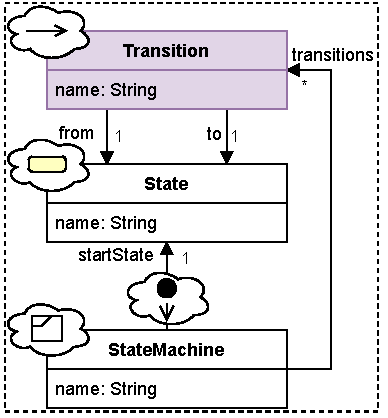
\includegraphics[width=0.275\textwidth]{figures/state_machine_metamodel.pdf}
    \caption{Finite state machine metamodel $M^1$}
    \label{fig:fsm_metamodel}
\end{figure}

A \textsf{StateMachine} has a \textsf{startState} and \textsf{transitions}, whereas each \textsf{Transition} connects two \textsf{State}s.
The states of a state machine are not explicitly modeled, but can be derived from the states connected by the transitions of a state machine.

Similarly, we must define a metamodel for the \gls*{bpmn} diagrams.
\autoref{fig:bpmn_metamodel} shows a simplified metamodel for \gls*{bpmn} (ignore the purple coloring for now).
Once more, we have attached concrete syntax elements.

% bpmn (subset of the needed constructs)
\begin{figure}[h]
    \centering
    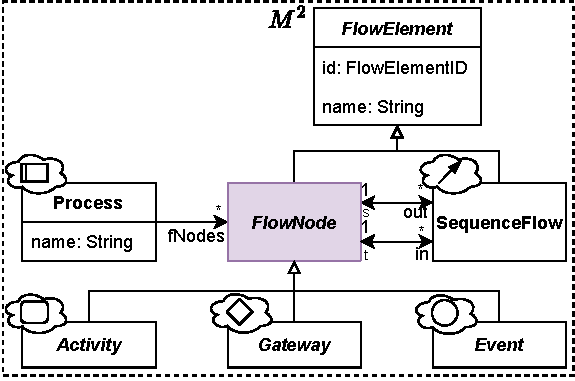
\includegraphics[width=0.475\textwidth]{figures/bpmn_metamodel.pdf}
    \caption{Simplified BPMN metamodel $M^2$ \cite{objectmanagementgroupBusinessProcessModel2013}}
    \label{fig:bpmn_metamodel}
\end{figure}

A \gls*{bpmn} \textsf{Process} contains a set of \textsf{FlowNode}s connected by \textsf{SequenceFlow}s.
A \textsf{FlowNode} can be an \textsf{Activity}, \textsf{Gateway}, or \textsf{Event}.
Possible \gls*{bpmn} \textsf{Gateway}s are shown in \autoref{fig:bpmn_gateways}.

\begin{figure}[h]
    \centering
    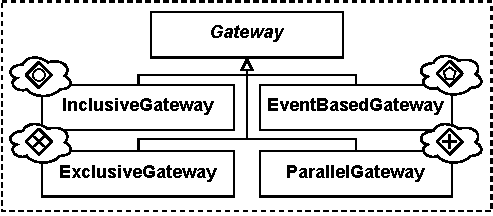
\includegraphics[width=0.4\textwidth]{figures/gateways.pdf}
    \caption{BPMN gateways \cite{objectmanagementgroupBusinessProcessModel2013}}
    \label{fig:bpmn_gateways}
\end{figure}

Similarly, specific activities and events are defined in the full \gls*{bpmn} metamodel \cite[Figure 10.6/10.69]{objectmanagementgroupBusinessProcessModel2013}.
The essential activities are manual tasks, service tasks, send/receive tasks, and call activities.
In the case of events, start events, message events, timer events, and end events are the most used.

\subsubsection{System relationship model}
We assume a set of behavioral models describing the system, which \emph{interact} to realize the global system behavior.
A system relationship model describes which behavioral models exist in the system and how they are related.
The system relationship \emph{metamodel} is depicted in \autoref{fig:systemRelationshipMetamodel}.

\begin{figure}[h]
    \centering
    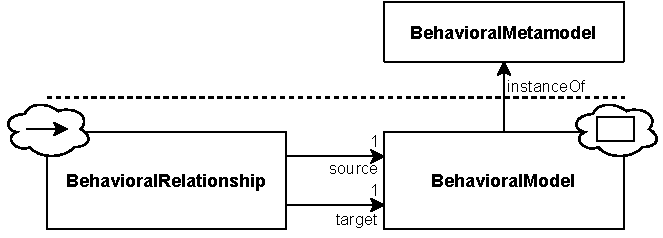
\includegraphics[width=0.45\textwidth]{figures/systemRelationshipMetamodel.pdf}
    \caption{System relationship metamodel \\ (without attributes and enumerations)}
    \label{fig:systemRelationshipMetamodel}
\end{figure}

Behavioral models typed in \textsf{BehavioralMetamodel}s can be connected by \textsf{BehavioralRelationship}s to allow for interactions.
We are using a \gls*{uml} class diagram-like syntax to define system relationship models, where each class corresponds to a behavioral model (typed in a \textsf{BehavioralMetamodel}), while each association corresponds to a \textsf{BehavioralRelationship} (see concrete syntax depicted in clouds).
Thus, a system relationship model does \emph{not} describe the structure of a system, but rather behavioral relationships between the behavioral models of a system.
The behavioral relationships will be crucial to define interactions between the models in the first step of our approach.

In addition, we allow enumerations and their use as attributes for behavioral models in the system relationship model.
This helps not to duplicate behavioral models because we can use the attributes as parameters, for example, to define the start state in a state machine (see \autoref{fig:systemInteractionModel}).
Different instances of the system relationship model can be used to analyze the global behavior of \emph{different} system configurations by changing the attribute values and behavioral model instances.

The system relationship model in the use case (see \autoref{fig:systemInteractionModel}) contains three classes corresponding to the traffic light, T-Junction, and Bus behavioral models.
A T-Junction has three relationships with the traffic light, which allows the T-Junction to interact with up to three traffic lights.
In addition, we can analyze different scenarios by adding buses approaching from particular directions.

% snapshot metamodel
\subsubsection{Snapshot metamodels}
The provided metamodels are used to structurally define all possible models by requiring a typing from each model to its metamodel.
In addition, we can add constraints to restrict all typed models further.

However, we need additional or different concepts from those in the metamodel to describe the structure of instances of the behavioral models during execution.
Consequently, we introduce a new model type called the \emph{snapshot metamodel}, which defines the structure of a state for a given formalism (see \autoref{fig:modelTypes}).

The snapshot metamodel for a state machine is straightforward, since a state machine can only be in one state at a time, as shown in \autoref{fig:fsm_snapshot_model}.
Since we are only interested in the current state and not the history of states, we call this a \emph{state machine snapshot}.
We are reusing the concrete syntax elements from the metamodel level.
In addition, each snapshot metamodel has a root element in our approach, highlighted in light blue in \autoref{fig:fsm_snapshot_model}.
\begin{figure}[h]
    \centering
    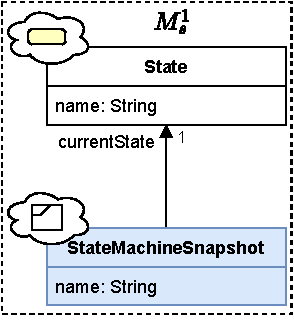
\includegraphics[width=0.22\textwidth]{figures/state_machine_s_model.pdf}
    \caption{Finite state machine snapshot metamodel $M_s^1$}
    \label{fig:fsm_snapshot_model}
\end{figure}

We define the snapshot metamodel for \gls*{bpmn} using tokens as suggested by the semantics description in \cite{objectmanagementgroupBusinessProcessModel2013}.
Thus, \autoref{fig:bpmn_snapshot_model} shows that a \emph{snapshot} of a process is a set of \textsf{Token}s.
If the set of \textsf{Token}s is empty, the state \textsf{Terminated} is derived.
Otherwise, the process is still \textsf{Running}.
Furthermore, \textsf{ProcessSnapshot}s can also have \textsf{subprocesses} with associated \textsf{Token}s.
A \textsf{Token} indicates where it is located in the \gls*{bpmn} using its \textsf{position} attribute.
A valid \textsf{position} is a sequence flow or a started but unfinished activity.

\begin{figure}[h]
    \centering
    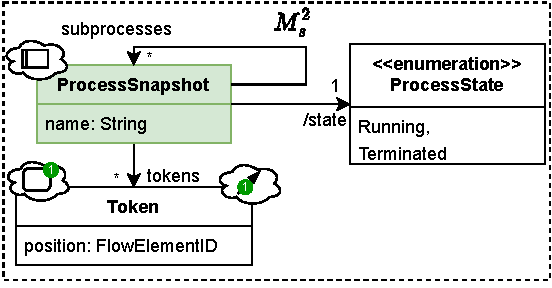
\includegraphics[width=0.475\textwidth]{figures/bpmn_s_model.pdf}
    \caption{BPMN snapshot metamodel $M_s^2$}
    \label{fig:bpmn_snapshot_model}
\end{figure}

\textsf{ProcessSnapshot}s are visualized using the concrete syntax of the underlying process.
In addition, \textsf{Token}s are highlighted with green bubbles in the middle of sequence flows or the top right of an activity.
The root of the \gls*{bpmn} snapshot metamodel is the \textsf{ProcessSnapshot}, highlighted in light green.

% Describe the remaining steps of the workflow in detail by/while applying them to the use case.
\subsection{Define model interactions}
Structural models in a multi-model might contain related information.
Thus, current approaches define so-called \emph{commonalities} to explicate these relationships and keep the information consistent \cite{stunkelComprehensiveSystemsFormal2021,klareCommonalitiesPreservingConsistency2019}.

To check the behavioral consistency of a system, we are primarily interested in the global system behavior.
However, global behavior depends not only on the local behavior of the models, but also on their interactions.
Consequently, we call these inter-model relationships \emph{interactions} since they carry behavioral meaning while commonalities carry structural meaning \cite{krauterBehavioralConsistencyHeterogeneous2021}.

To specify interactions between different behavioral models, we defined an interaction language given by the interaction metamodel in \autoref{fig:interaction_metamodel}.
The interaction metamodel uses concepts from the system relationship metamodel (see \autoref{fig:systemRelationshipMetamodel}) since interactions can only be specified between behavioral models connected by \textsf{BehavioralRelationship}s.

In addition, we introduce the concept of \emph{state-changing elements}.
Each \textsf{BehavioralMetamodel} specifies a set of \textsf{StateChangingElement}s.
For example, a state machine defines states and transitions, but only the transitions describe how the states in a state machine change.
Thus, the transitions are the \textsf{StateChangingElement}s of a state machine (highlighted in purple, see \autoref{fig:fsm_metamodel}).
Similarly, the flow nodes are the \textsf{StateChangingElement}s of a \gls*{bpmn} process (highlighted in purple, see \autoref{fig:bpmn_metamodel}).
The interaction of behavioral models is only possible through instances of the \textsf{StateChangingElement}s.

\begin{figure}[h]
    \centering
    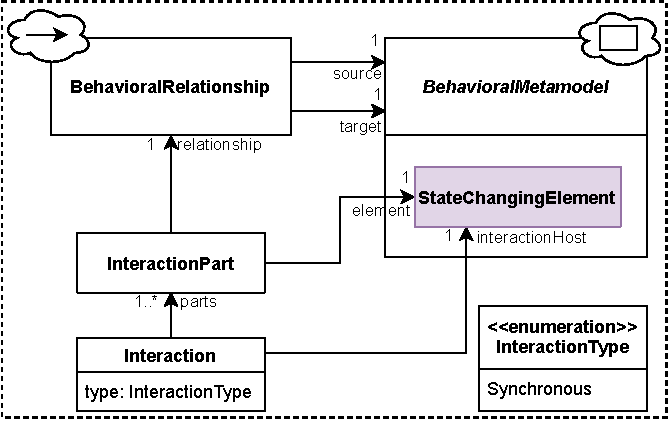
\includegraphics[width=0.475\textwidth]{figures/interaction_metamodel.pdf}
    \caption{Interaction metamodel}
    \label{fig:interaction_metamodel}
\end{figure}

An \textsf{Interaction} has an \textsf{interactionHost} and a set of interaction \textsf{parts}.
Each \textsf{InteractionPart} references one \textsf{BehavioralRelationship} and one \textsf{StateChangingElement}.
Again, we attach some concrete syntax elements to the interaction metamodel, which we use to define interactions later.

The \textsf{interactionHost} and the elements of the \textsf{InteractionPart}s describe a state change for their concrete behavioral model.
By connecting them with an interaction, we define that all state changes must happen simultaneously in one atomic step.
Consequently, the interactions define synchronizations of the behavioral models.
In addition, each \textsf{InteractionPart} must be based on a \textsf{BehavioralRelationship} in the system relationship model, which must have the behavioral model containing the \textit{interactionHost} as a source and the behavioral model containing the \textsf{StateChangingElement} of the \textsf{InteractionPart} as a target.
Thus, one can only define interactions for behavioral models connected by behavioral relationships.

We allow the definition of as many interactions as desired.
The interactions restrict the local behavior of the models since some parts of its behavior must synchronize, i.e., certain behavior cannot happen locally anymore.
If two interactions share elements that should be synchronized, the interactions do not influence each other, such that either of them can happen.

% causality/asynchronous communication can be defined using synchronous communication and an intermediate model
Currently, interactions only specify synchronization and not causality between models, i.e., this state change should happen before/after the other one.
However, causality between state changes can be modeled using only synchronization.
% A --> B. A synchronizes with a state-changing element in new intermediate behavioral model (acting as a buffer).
% The subsequent element in the new behavioral model synchronizes with B.
In the future, one could support causality directly, effectively introducing \emph{syntactic sugar} for interactions.

In the use case, the T-Junction controller interacts with the three traffic lights, \textbf{A}, \textbf{B}, and \textbf{C}.
\autoref{fig:interactions} depicts this interaction (cyan-colored parts) synchronizing the traffic lights with the T-Junction controller.
It has three \textsf{InteractionPart}s specifying the synchronization with each traffic light.
We are using the concrete syntax of interactions, defined in the interaction metamodel (see \autoref{fig:interaction_metamodel}).

\begin{figure}[h]
    \centering
    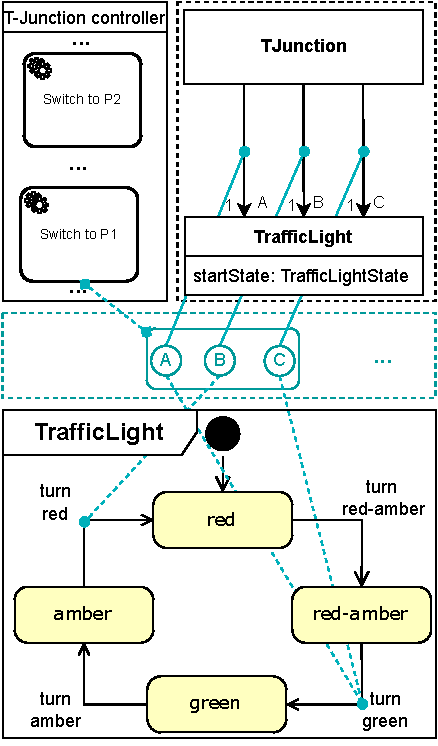
\includegraphics[width=0.35\textwidth]{figures/interactions.pdf}
    \caption{One interaction for the use case}
    \label{fig:interactions}
\end{figure}

We can explain the interaction as follows.
The connection of the interaction to the task \textsf{Switch to P1} defines that the execution of the task in a \textsf{T-Junction controller} should be part of a synchronization.
\textsf{Switch to P1} is the interaction host and its behavioral model the \textsf{TJunction} is connected with the traffic lights in the system relationship model.
Furthermore, the three bubbles and their connections to the two other models state which transitions of which traffic lights should participate in the synchronization.
For example, bubble \textbf{A} determines that a \textsf{TrafficLight} connected by an A-typed behavioral relationship should be present and \textsf{turn green} simultaneously with the execution of the task.
A corresponding interaction exists for the activity \textsf{Switch to P2} but is not shown in \autoref{fig:interactions}.

\subsection{Generate execution semantics} \label{subsec:executionSemantics}
To execute the models, we must be able to represent the global system state, which is composed of the individual states of each behavioral model.
We call this model the \emph{global snapshot metamodel}.

To calculate the global snapshot metamodel, one must merge all snapshot metamodels with the system relationship model.
The first step is to add all model elements to one global model, i.e., calculating their disjoint\footnote{Possible conflicts due to the naming of model elements can be resolved by user input or a fixed strategy, for example, prefixing model elements with the model name.} union.

The second step is adding inheritance relations to connect behavioral models in the system relationship model with their corresponding snapshot metamodels.
Each behavioral model is typed in a behavioral metamodel, which has a snapshot metamodel (\autoref{fig:modelTypes}) structurally describing its state.
Thus, we know how the states of each behavioral model are structured by referring to its metamodel.
We make this knowledge explicit by adding an inheritance relation for each behavioral model to the root of the corresponding snapshot metamodel.
The resulting artifact, the \emph{global snapshot metamodel}, describes all possible states of the global system, since each behavioral model inherits a description of its state.

\autoref{fig:global_execution_model} depicts the global snapshot metamodel $M_s^+$ for the use case, describing the states of the traffic management system.
We added three inheritance relations to construct $M_s^+$ for the use case and omitted unchanged parts from the system relationship model and the individual snapshot metamodels.

\begin{figure}[h]
    \centering
    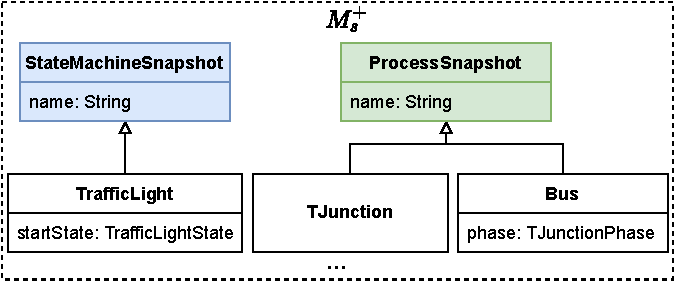
\includegraphics[width=0.475\textwidth]{figures/global_s_model.pdf}
    \caption{Global snapshot metamodel $M_s^+$ for the use case}
    \label{fig:global_execution_model}
\end{figure}

With the global snapshot metamodel, we can represent the global states of the system, but we still need execution semantics to generate a state space to check the properties.
The execution semantics used in our approach must fulfill the following three requirements:
\begin{enumerate}
    \item The execution semantics must incorporate each behavioral model.
    \item The execution semantics must reflect the defined interactions between the behavioral models.
    \item The execution semantics must generate a state space, where each state is an instance of $M_s^+$, given a system configuration (instance of the system relationship model).
\end{enumerate}
Generally, our approach is independent of the underlying execution semantics if it fulfills the three requirements.
Thus, one can experiment with different underlying semantics, for example, graph transformations, state machines, Petri nets, or process algebras, without changing the general framework.
One can then pick the most suitable semantics for the modeling scenario at hand regarding, for example, consistency checking performance.

To summarize, we obtain execution semantics, which describes the global behavior of the system.
Generating these execution semantics from the models and interactions must be fully automated to allow frequent model changes.
Later in the paper, we introduce execution semantics based on graph transformations and apply them to the use case.

\subsection{Check behavioral consistency}
We use the previously constructed execution semantics for consistency checking to generate a state space based on a system configuration.
However, we also need atomic propositions interpreted on the global states to define and check global properties.

Atomic propositions must be formulated uniformly for all used behavioral models.
We propose to use the global snapshot metamodel $M_s^+$ to formulate atomic propositions by providing an instance of it for each atomic proposition.
\autoref{fig:atomic_propositions} shows how to formulate the atomic propositions $A_{green}$ and $B1_{passing}$, used in the global properties, stated earlier.
Varying propositions with more or less complexity can be formulated using this approach.

\begin{figure}[h]
    \centering
    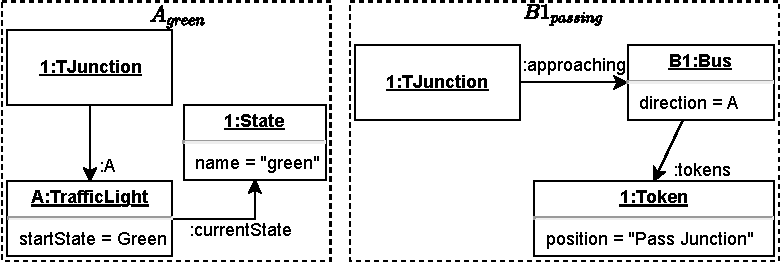
\includegraphics[width=0.475\textwidth]{figures/atomic_props.pdf}
    \caption{Atomic propositions $A_{green}$ and $B1_{passing}$}
    \label{fig:atomic_propositions}
\end{figure}

Since each state is an instance of $M_s^+$, we can interpret the constructed atomic propositions on the states.
An atomic proposition is true for a state if the corresponding instance of $M_s^+$ contains the atomic proposition.
Then, we can check consistency requirements on the generated state space.
This step should be fully automated, such that it can be executed as many times as needed (indicated by the loop in \autoref{fig:approach}) for different system configurations and consistency requirements (including atomic propositions).

Alternatively, to make formulating atomic propositions less cumbersome, one can use the concrete syntax of the individual snapshot metamodels to formulate atomic propositions.
For example, \autoref{fig:atomic_propositions_concrete} shows the same atomic propositions as \autoref{fig:atomic_propositions} but uses the introduced concrete syntax.

\begin{figure}[h]
    \centering
    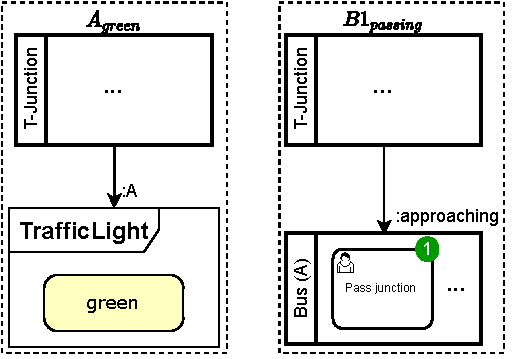
\includegraphics[width=0.4\textwidth]{figures/atomic_props_concrete.pdf}
    \caption{Concrete syntax for $A_{green}$ and $B1_{passing}$}
    \label{fig:atomic_propositions_concrete}
\end{figure}

Finally, if a consistency requirement is violated, a counterexample based on the state space should be presented to the user.
An unsuccessful consistency check leads to a consistency restoration process, which is crucial but out of scope for this contribution.
We describe consistency checking for the use case and its result in the next section.
In addition, the appendix contains \autoref{fig:allConcepts}, which gives an overview of the introduced concepts and their usage.

\section{Maude execution semantics} \label{sec:maude_execution_semantics}

% TODO: Briefly describe maude execution semantics

\section{Related work} \label{sec:related_work}
This contribution builds on our previous publication \cite{krauterBehavioralConsistencyHeterogeneous2021}.
However, we refined the behavioral consistency management workflow by introducing new concepts such as the system relationship model and snapshot metamodel.
Moreover, we created an interaction language and outlined a general approach to define atomic propositions, leading to global behavioral properties.
In addition, our previous work did not support \gls*{bpmn} models.

% Highlight some specific combinations/ad-hoc approaches for a single modeling language.
The general idea of transforming different behavioral formalisms to a single semantics domain to reason about cross-cutting concerns is not new, see, e.g. \cite{engelsMethodologySpecifyingAnalyzing2001}.
For example, \cite{kusterExplicitBehavioralConsistency2003} developed consistency checking for sequence diagrams and statecharts based on \gls*{csp}, while \cite{yaoConsistencyCheckingUML2006} used Petri nets for the same scenario.
Furthermore, \cite{cunhaFormalVerificationUML2011} analyze sequence diagrams in the context of embedded systems using a transformation to Petri nets.
Nevertheless, all approaches focus on a single modeling language or a fixed combination of two languages.
Consequently, they do not consider the general problem of behavioral consistency in a heterogeneous modeling scenario.

% Kienzle with event structures
\cite{kienzleUnifyingFrameworkHomogeneous2019} proposes a unifying framework for homogeneous model composition.
To combine behavioral models, they use Event structures \cite{winskelEventStructures1987} as an underlying formalism and show how different homogeneous behavioral models can be combined.
Nonetheless, they do not apply their approach to heterogeneous models.
Generally, their approach is compatible with ours, since we do not mandate a specific formalism in our approach.
However, we have chosen graph production rules as the first formalism to use in our approach, since they operate on a higher abstraction level.
In addition, it was shown that many formalisms, for example, the $\pi$-calculus \cite{gadducciGraphRewritingPcalculus2007}, can be implemented using graph production rules.

% Gemoc Studio/BCOOL?
% Approach is quite technical (i.e. execution engine. No formal execution semantics?)
\cite{deantoniModelingBehavioralSemantics2016} tackles the problem of dealing with relationships between heterogeneous behavioral models.
They coordinate the different models using their coordination language B-COoL \cite{varalarsenBCoolBehavioralCoordination2016}, similar to the interactions we define between behavioral models.
To execute the models and their coordination, they transform them into \gls*{ccsl} models.  
Their work also results in plugins for GEMOC studio, which support running and debugging the models.
% Ptolemy
\cite{ekerTamingHeterogeneityPtolemy2003, leeDisciplinedHeterogeneousModeling2010} propose an actor-oriented solution to the model composition problem in the presence of heterogeneity.
Their approach results in the tool Ptolemy \cite{ptolemaeusSystemDesignModeling2014}.

% very nice, but only simulation for Ptolemy and no real verification support (LTL model checking and atomic prop definition) in BCool/Gemoc.
However, both approaches focus on simulation rather than consistency or model-checking.
Neither provides concrete means to define atomic propositions and check global behavioral properties.

\section{Evaluation \& State space explosion}
% TODOS:
% - Generally we not only support model checking but also simulation.
% - Real-time systems can also be checked using maude. This could be mentioned somewhere and the oslo papers can be cited.

% Evaluation against other approaches not done yet but part of future work.
% Evaluate the maude and GT implementation. Maybe start with the maude one.
% What do we evaluate? Runtime and scalability i.e. state space explosion.
State space explosion is one of the predominant issues when applying model checking to complex systems as they are often found in real-world applications.
In this section, we will briefly evaluate and discuss our approach in terms of scalability to estimate the effect of state space explosion.
We start with the multi-model from the use case and then increase the number of approaching buses to simulate growing complexity.
\autoref{table:runtime} shows the results of our experiments.

% Preliminary numbers on the laptop. Need some explanation for them
% Adding buses is quite bad since they nearly run independent from the rest. And we are doing a full state space exploration.
% Partial order reduction would have huge potential here.
% Cite comparable performance with Spin?
% Maude is single threaded but interesting queries can be run in parallel.
% This should be faster on a desktop or even stronger server CPU. Can be run during CI/CD. At least the most expensive ones.
\begin{table}
\centering
\begin{tabular}{|c || c | c | c |}
 \hline
 Use case & States & Rewrites & Exploration time \\
 \hline\hline
 No buses & 168 & 663 & ~10 ms \\
 \hline
 1 bus & 3.304 & 20.117 & ~190 ms \\
 \hline
 2 buses & 67.624 & 549.509 & ~5.500 ms \\
 \hline
 3 buses & 716.912 & 7.183.505 & ~69.600 ms \\
 \hline
\end{tabular}
\caption[Model checking runtime]{Model checking runtime\footnotemark}
\label{table:runtime}
\end{table}

% TODO: Fill in real specs.
\footnotetext{The results were obtained using a machine with X processor and Y GB of RAM running Maude version 3.2.1.
A description how to run the experiment can be found at \cite{timkrauterBehavioralConsistencyMultimodeling2022}.}

% Discuss the results and talk about ways to mitigate state space explosion.
The results in \autoref{table:runtime} were obtained without applying any optimization techniques.
The Maude LTL model-checker has performance comparable to the popular SPIN model checker \cite{ekerMaudeLTLModel2004}.
In the future, one could use different techniques to further mitigate the state space explosion problem.
One technique is to abstract models further such that they only contain information relevant for the set of properties to be checked.
Thus, minimal models are synchronized leading to smaller state spaces.
However, finding correct minimal models might not be trivial.

Partial-order reduction is a well-known and successful technique to mitigate the state space explosion problem.
It is currently not implemented in the Maude LTL model-checker but there is promising work to integrate partial-order reduction into the model-checker \cite{farzanPartialOrderReduction2007}.
The potential to reduce the state space using this technique is huge, especially for model-checking concurrent systems \cite{clarkeHandbookModelChecking2018}.
The systems our approach analyzes are concurrent systems with some interaction.

% Discuss state space explosion
% Obviously, it is a problem. Especially the more behaviors are interacting.
% However, if you want to check a global behavior, all individual behaviors are needed (to a certain degree)

% Huge potential for partial order reduction to reduce the state space. Why?
% Might already be implemented in Maude! We should finish the implementation and make some tests!
\section{Conclusion and future work} \label{sec:conclusion_and_future_work}
% Conclusion
Our work represents the first general fully-formalized approach to behavioral consistency management in a heterogeneous modeling scenario, enabling formulating and checking \emph{global} properties.
Previous work either only dealt with the behavioral consistency between specific pairs of models \cite{yaoConsistencyCheckingUML2006, kusterExplicitBehavioralConsistency2003} or focused on the simulation in a heterogeneous scenario \cite{deantoniModelingBehavioralSemantics2016, varalarsenBCoolBehavioralCoordination2016, ekerTamingHeterogeneityPtolemy2003, leeDisciplinedHeterogeneousModeling2010}.

Our approach follows three key steps (see \autoref{fig:approach}).
% Describe the three steps
First, we align the behavioral models by defining their interactions.
Then, we generate global execution semantics based on the defined interactions while preserving the original behavior of the models.
Finally, we can check the global consistency of the system in different configurations with varying consistency requirements using the generated semantics.
Although our approach is independent of a particular formalism as an underlying global execution semantics, the current implementation utilizes graph transformations for this purpose.

% Future work:
Since we could not fully describe our formalization of the \gls*{bpmn} semantics using graph transformations, we plan to do so in a future publication, including a thorough comparison with other formalizations such as \cite{vangorpVisualTokenbasedFormalization2013} and \cite{dijkmanSemanticsAnalysisBusiness2008}.

It is also interesting to extend the graph transformation execution semantics to include other behavioral formalisms such as activity diagrams, hierarchical state machines, and the $\pi$-calculus.
Especially integrating the $\pi$-calculus, which was formalized using graph grammars in \cite{gadducciGraphRewritingPcalculus2007}, will be beneficial since it is profoundly different from the currently supported formalisms.
% Should write about data transfer between systems as future work (and things which are not supported yet by other formalisms). I guess we need a general model and map from/to it during interactions. Each formalism would have to implement some mapping from and to this universal model once. But we do not need mappings between all formalisms directly. This can be implemented using equations in maude or something like that.
% Could write about a different implementation than gt. Maybe a spin code generation for more scalable model checking.
% Could write about continuous time models to be included in the future.

\bibliography{bib}
\section*{About the authors}

\shortbio{Tim Kräuter}{is a Ph.D. research fellow at the Western Norway University of Applied Sciences, Bergen, Norway.
His primary research is on integrating heterogeneous behavioral models in multi-model-driven software engineering.
Previously he worked as a software developer at SET GmbH in Germany and acquired a master of science in Information Engineering at the University of Applied Sciences, FHDW Hannover, Germany.
\authorcontact[https://timkraeuter.com/]{tkra@hvl.no}}

\shortbio{Harald König}{is a professor for Computer Science at the University of Applied Sciences, FHDW Hannover, Germany, and an Adjunct Professor at the Department of Computer Science, Electrical Engineering and Mathematical Sciences at the Western Norway University of Applied Sciences, Bergen, Norway.
Before entering academia, he worked at SAP in Walldorf and received his Ph.D. in pure Mathematics from Leibniz University in Hannover, Germany. \authorcontact{harald.koenig@fhdw.de}}

\shortbio{Adrian Rutle}{is a professor at the Department of Computer science, Electrical engineering and Mathematical sciences at the Western Norway University of Applied Sciences, Bergen, Norway.
Rutle’s main interest is applying theoretical results from the field of model-driven software engineering to practical domains and has his main expertise in the development of formal modeling frameworks for domain-specific modeling languages, graph-based logic for reasoning about static and dynamic properties of models, and the use of model transformations for the definition of the semantics of modeling languages.
His recent research focuses on multilevel modeling, model repair, multi-model consistency management, modeling and simulation for robotics, digital fabrication, smart systems, and applications of machine learning in model-driven software engineering.
\authorcontact{aru@hvl.no}}

\shortbio{Yngve Lamo}{is a professor at the Department of Computer science, Electrical engineering and Mathematical sciences at the Western Norway University of Applied Sciences, Bergen.
Lamo holds a Ph.D. in Computer Science from the University of Bergen, Norway. His research interests span from formal foundations of Model Based Software Engineering to its applications, especially in Health Informatics.
He is currently applying MDSE to create Adaptive Software Technologies for mental Health. \authorcontact{yla@hvl.no}}

\shortbio{Patrick Stünkel}{is currently working as a postdoctoral researcher at Haukeland University Hospital in Bergen, Norway, where he is working on applying process mining, workflow modeling, and optimization techniques in digital pathology.
Before that, Patrick did his Ph.D. at Western Norway University of Applied Sciences on the topics of semantic interoperability and consistency management among heterogeneous software models.
\authorcontact[https://past.corrlang.io/]{Patrick.Stunkel@helse-bergen.no}}

\begin{figure*}[h]
    \centering
    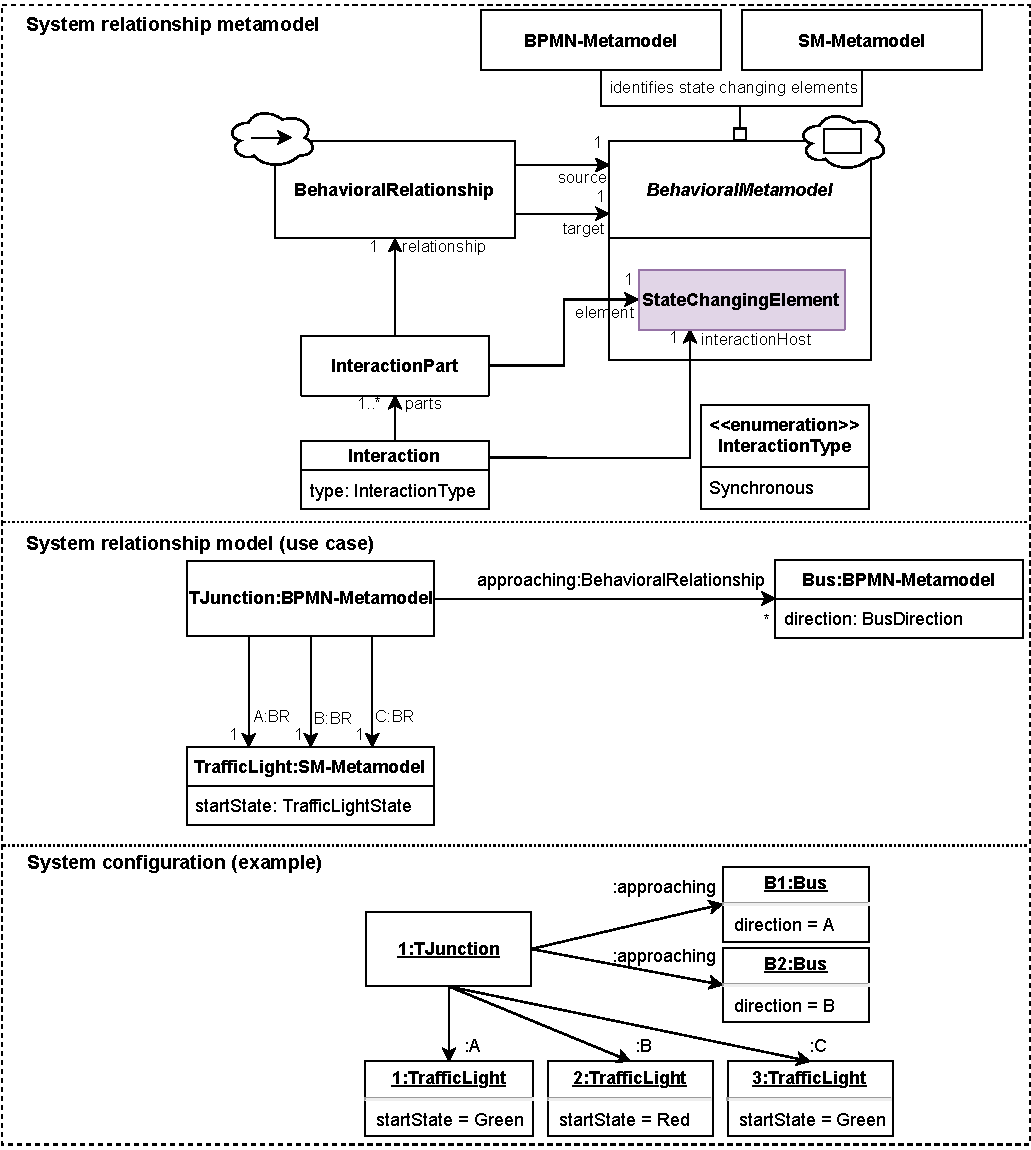
\includegraphics[width=1\textwidth]{figures/allConcepts.pdf}
    \caption{Overview of all concepts and their use in the system relationship model}
    \label{fig:allConcepts}
\end{figure*}

\end{document}